\documentclass[10pt,a4paper,titlepage]{article}
\usepackage[utf8]{inputenc}
\usepackage{amsmath}
\usepackage{amsfonts}
\usepackage{amssymb}
\usepackage{makeidx}
\usepackage{enumitem}
\usepackage{graphicx}
\usepackage{longtable}
\usepackage[hidelinks]{hyperref}

%this is a command used in the title template
\newcommand{\HRule}{\rule{\linewidth}{0.5mm}}

%questo fa in modo che le liste numerate siano allineate come le altre
\setenumerate{leftmargin=*, labelindent=\parindent}

%questo genera il toc, ricorda di eseguire due volte
\makeindex

\begin{document}
\begin{titlepage}
\begin{center}

%logo

\includegraphics[width=0.30\textwidth]{./images/logo}~\\[1cm]
\textsc{\LARGE Politecnico di Milano}\\[1.5cm]

\textsc{\Large Software Engineering 2 Project}\\[0.5cm]

% Title
\HRule \\[0.4cm]
{ \Huge \bfseries MeteoCal \\[0.4cm] }
{ \huge \bfseries Design Document \\[0.4cm] }
\HRule \\[1.5cm]

% Author
\begin{flushright}
\noindent
\large
\emph{Authors:}\\
Andrea \textsc{Celli}\\
Stefano \textsc{Cereda}
\end{flushright}
\vfill

% Bottom of the page
{\large \today}

\end{center}
\end{titlepage}

\part{Introduction}
\label{part:introduction}

\section{Purpose of this document}
This document describes the general and specific architecture of MeteoCal, the project of the course of Software Engineering 2 at Politecnico di Milano.
The document will explain the architectural decisions and trade offs chosen in the design process and its justifications.

\section{Scope}
The architectural descriptions provided concern the functional view, module view, deployment view, data layer, business logic and the user interface of the RASD.
Hence the architecture will consider the following functionalities offered by MeteoCal:

\begin{itemize}
\item \emph{Users:} MeteoCal will manage personal data of the users. MeteoCal will manage registering, logging in/out and the modification of personal data.

\item \emph{Calendars:} MeteoCal will manage a calendar for each user. User will be able to create, update and delete an event and to see other people's events. MeteoCal will also manage event invitation and notifications for the event's update.

\item \emph{Weather:} MeteoCal will manage weather forecasts and send notifications to event's participants one day in advance in case of bad weather. It will also have to propose an alternative schedule to the event creator with three day of advance.
\end{itemize}

\section{Definitions and acronyms}

\subsection{Definitions}

\begin{itemize}
\item \emph{Calendar:} a calendar is the agenda of an user
\item \emph{Event:} a task that a user has into his calendar
\item \emph{Registered user:} a user that has created an account on MeteoCal
\item \emph{Logged user:} a registered user that has performed the login process
\item \emph{Unlogged user:} either a non registered user or a registered user that is logged out of the system
\item \emph{Participant:} a participant to an event is either its creator or an invited user who accepted the invite
\item \emph{Bad weather alert:} the notification send to the user with one day of advance if weather forecasts for outdoor events on the next day are bad
\item \emph{Date changed notification:} the notification send to every participant if the event creator change the event date
\item \emph{System:} the MeteoCal system
\end{itemize}

\subsection{Acronyms and abbreviations}
\begin{itemize}
\item \emph{MeteoCal:} Meteorological Calendar
\item \emph{G:} Goal
\item \emph{JVM:} Java Virtual Machine
\item \emph{JEE:} Java Enterprise edition
\item \emph{DBMS:} Database management system
\item \emph{AS:} Application server
\item \emph{FR:} Functional requirement
\item \emph{NFR:} Non-functional requirement
\item \emph{BWA:} Bad weather alert
\item \emph{DCN,ECN:} Date-Event changed notification
\item \emph{SDP:} Sunny day proposal 
\end{itemize}

\section{References}
\begin{itemize}
\item Analysis document: \url{./RASD.pdf}
\end{itemize}

\section{Overview}
This document specifies the architecture of MeteoCal spreading from the general into the specific. It also describes and justifies the architectural decisions and trade offs.
The design was guided by a top-down process approach and the document structure reflects this tactic.

The document is organized as follows:
\begin{itemize}
\item \emph{Part \ref{part:introduction}, Introduction:} provides a synopsis of the architectural descriptions.
\item \emph{Part \ref{part:design-overview}, Design Overview:} provides a general description of MeteoCal including its functionality and matters related to the overall system and its design.
\item \emph{Part \ref{part:design-considerations}, Design Considerations:} describes the design assumptions and constrains of MeteoCal.
\item \emph{Part \ref{part:software-architecture}, Software Architecture:} specifies the general architecture, describes the basic structure and interactions of the main subsystems.
\item \emph{Part \ref{part:detailed-software-design}, Detailed System Design:} specifies in detail the components of the system through different architectural views.
\item \emph{Part \ref{part:appendixes}, Appendixes:} provides supporting information and additional material.
\end{itemize}

\clearpage
\part{Design overview}
\label{part:design-overview}
This section provides a general description of the software system including its functionality and concerns related to the overall system and its design.

\section{Design context}
The design context sets the limits for the system design, considering the functional and technological context.

\subsection{Functionalities}
The following functional requirements were identified in the RASD. These functionalities are grouped by the following functional areas:

\subsubsection{Managing users}
Functional requirements:
\begin{enumerate}[label = FR \arabic*:]
\item Register to system
\item Login
\item Logout
\item Modify password
\item Recover password
\item Update personal data
\end{enumerate}

\subsubsection{Managing calendars}
Functional Requirements:
\begin{enumerate}[label = FR \arabic*:]
\setcounter{enumi}{6}
\item Add a new event
\item Modify an existing event
\item Delete an existing event
\item View your own schedule 
\item View the details of your own event
\item Send an invitation to other users
\item Reply to an invitation
\item See the schedule of other users if their calendar is public
\item See the details of other user's public events
\item Receive a notification when the event details changes
\end{enumerate}

\subsubsection{Managing weather forecasts}
Functional requirements:
\begin{enumerate}[label = FR \arabic*:]
\setcounter{enumi}{16}
\item Send a notification the day before an event in case of bad weather to all the event's participants
\item Propose an alternative schedule three days before an event in case of bad weather to the event creator
\item Show the weather forecasts for the scheduled events 
\end{enumerate}

\subsection{System technologies}
MeteoCal will be designed considering the client-server 3-tier distributed architectural style as depicted in figure \ref{fig:JEE_arch}. Each tier requires specific technologies as depicted below.
\begin{figure}[ph]
\centering
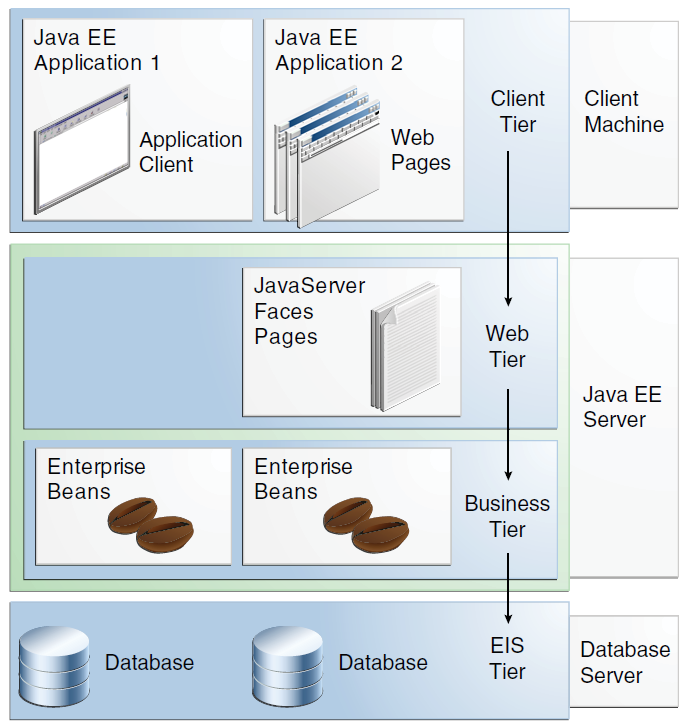
\includegraphics[width=\linewidth]{./images/JEE-arch}
\caption[jee arch]{JEE architecture}
\label{fig:JEE_arch}
\end{figure}


\subsubsection{Web tier}
\begin{itemize}
\item Dynamic web pages containing XHTML, which are generated by web components.
\item Web components developed with Java Server Faces technology, which is a user interface component framework for web applications.
\end{itemize}

\subsubsection{Business logic tier}
\begin{itemize}
\item Java Enterprise Edition 7(JEE7) platform supports applications that provide enterprise services in the Java language. It is the common foundation for the various kinds of components in Java.
\item Enterprise Java Beans (EJB) 3.1, business components that capture the logic that solves or meets the needs of a particular business domain and persistence entities.
\item GlassFish 4.1, a server that provides services such as security, data services, transaction support, load balancing, and management of distributed applications and supports the JEE7 platform.
\end{itemize}

\subsubsection{Persistence tier}
\begin{itemize}
\item MySQL Server 5.6.21, a RDBMS
\end{itemize}

\section{General design description}
This section presents the road map followed to model the architecture of MeteoCal, including its functionality and matters related to the overall system and its design.

\subsection{Design approach}
The design approach is based on a client-server 3-tier distributed system, where each tier is described as follows:
\begin{itemize}
\item \emph{Client tier:} This tier is responsible of translating user actions and presenting the output of tasks and results into something the user can understand.
\item \emph{Business Logic tier:} This tier coordinates the application, processes commands, makes logical decisions and evaluations, and performs calculations. It also moves and processes data between the client and the persistence tiers.
\item \emph{Persistence tier:} This tier holds the information of the system data model, and is in charge of storing and retrieving information from a database. 
\end{itemize}

The design process followed a top-down process approach, so the outermost tiers were first identified and then broken into components that encapsulate the functionality. Hence each component is responsible for certain functionalities and interacts with others.

\subsection{Overall design}
This subsection presents the design model of MeteoCal, specifying the basic relations between packages, use cases and users.

\subsubsection{General package design}
Since each tier is broken into components and each component is responsible for a set of functionalities that fulfill the requirements, there is a correlation between use cases (functionality) and package design. In the diagram we can identify three packages:
\begin{itemize}
\item \emph{User UI:} This package contains the user interfaces. It is responsible for the interaction with the user such as getting UI requests, referring them to the Business Logic package and retrieving the data back for displaying.
\item \emph{Business Logic:} This package contains the business logic components. This package is responsible for handling the User UI package requests, processing them and accessing the Persistence package if required to provide a response.
\item \emph{Persistence:} This package is responsible for managing the data requests from the Business Logic package.
\end{itemize}

Logged and unlogged users access directly the User UI package and submit requests to accomplish their tasks.

\begin{figure}[h]
\centering
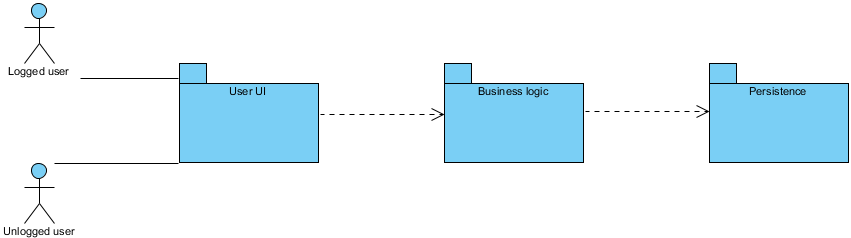
\includegraphics[width=\linewidth]{./images/basic-package}
\caption[Basic package]{Basic package diagram}
\label{fig:basic-package}
\end{figure}

\subsubsection{Detailed package design}
Given the functional requirements identified we can encapsulate them within specific components in the package diagram as follows:

\paragraph{User UI}
These set of sub packages are responsible for encapsulating the user actions and forwarding information requests to the Business logic sub packages.
\begin{itemize}
\item \emph{Login page:} this package implements FR2, FR5
\item \emph{Sign up page:} this package implements FR1
\item \emph{Calendar page:} this package implements FR3, FR7-FR12, FR14, FR15, FR19
\item \emph{Notification viewer:} this package implements FR13, FR16-FR18
\item \emph{User profile page:} this package implements FR4-FR6
\end{itemize}

\paragraph{Business logic}
These set of sub packages are responsible for handling requests from the User UI package, processing them and send back a response. These packages may access the Persistence package.
\begin{itemize}
\item \emph{Login manager:} this package implements FR2, FR3
\item \emph{User profile manager:} this package implements FR1, FR4-6
\item \emph{Calendar manager:} this package implements FR7-FR11, FR14, FR15
\item \emph{Search manager:} this package implements FR12, FR14, FR15
\item \emph{Notification manager:} this package implements FR13,FR16-FR19
\item \emph{Forecast manager:} this package implements FR17-FR19
\end{itemize}

\paragraph{Persistence}
This sub package contains the data model for the system. It accepts requests from the Business Logic package.
\begin{itemize}
\item \emph{Entity manager:} This package implements FR1-FR19
\end{itemize}

\begin{figure}[h!]
\centering
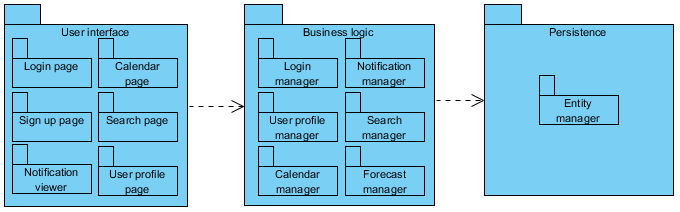
\includegraphics[width=\linewidth]{./images/detailed-package}
\caption[Detailed package]{Detailed package diagram}
\label{fig:detailed-package}
\end{figure}

\clearpage
\part{Design considerations}
\label{part:design-considerations}
This section encompasses the design considerations taken into account in the MeteoCal system design. Assumptions, dependencies, general constraints and performance requirements are clearly stated.

\section{Dependencies}
\begin{tabular}{| p{0.3\linewidth} | p{0.7\linewidth} |}
\hline	\emph{Dependency}	&	\emph{Impact}	\\
\hline	Java virtual machine that supports JEE7 is already installed on the OS. & MeteoCal only runs on operating systems that support the JEE7 platform.	\\
\hline	The supported browsers will be Firefox and Chrome & MeteoCal outputs XHTML code that requires browsers that support most of the web standards, elsewhere the UI experience will be affected.	\\
\hline	A JEE7 AS is required on the server side	&	MeteoCal cannot operate if there is no AS that supports the JEE7 standard	\\
\hline
\end{tabular}

\section{General constraints}
This section describes the NFRs and the QoS details related to the design of the software product.

\noindent\begin{tabular}{| l | l |}
\hline	\emph{Element}	&	\emph{Requirement}	\\
\hline	Memory			&	2 GB+				\\
\hline	Database server	&	MySQL				\\
\hline	Network			&	Internet access, HTTP protocol	\\
\hline	Security		&	User data will be encrypted. SSL is not supported	\\
\hline	Hard disk space	&	40 GB+				\\
\hline
\end{tabular}

\section{Performance requirements}
\subsection{Standard compliance}
The software product does not have to meet any standard compliance.

\subsection{Reliability}
For assuring the reliability of the software product, it is mandatory to back up the database periodically.

\subsection{Availability}
An AS is used to guarantee the availability of the software product. In a real scenario some redundancy in the AS instances is recommended, however here we will assume that all the tiers run on the same physical server.

\subsection{Security}
The software product does not support SSL in AS. It supports the hashing of the user password according to sha5 algorithm in the database. It supports authorization according JAAS.

\subsection{Maintainability}
The architectural style and the component definition described contribute to low coupling and high cohesion of the software product.

\subsection{Portability}
The software product will be developed using the Java language and related dependent technologies. Java is specifically designed to have as few implementation dependencies as possible. Meaning that code that runs on one platform does not need to be recompiled to run on another.

\clearpage
\part{Software architecture}
\label{part:software-architecture}
MeteoCal will be developed using a 3-tier JEE architecture. We have identified the components of each tier. Section \ref{sec:conceptual-design} gives a brief description of the architecture we will adopt to develop MeteoCal and a small description for each component. A detailed description will be provided in part \ref{part:detailed-software-design}.

\section{Conceptual design}
\label{sec:conceptual-design}
\begin{figure}[htp]
\centering
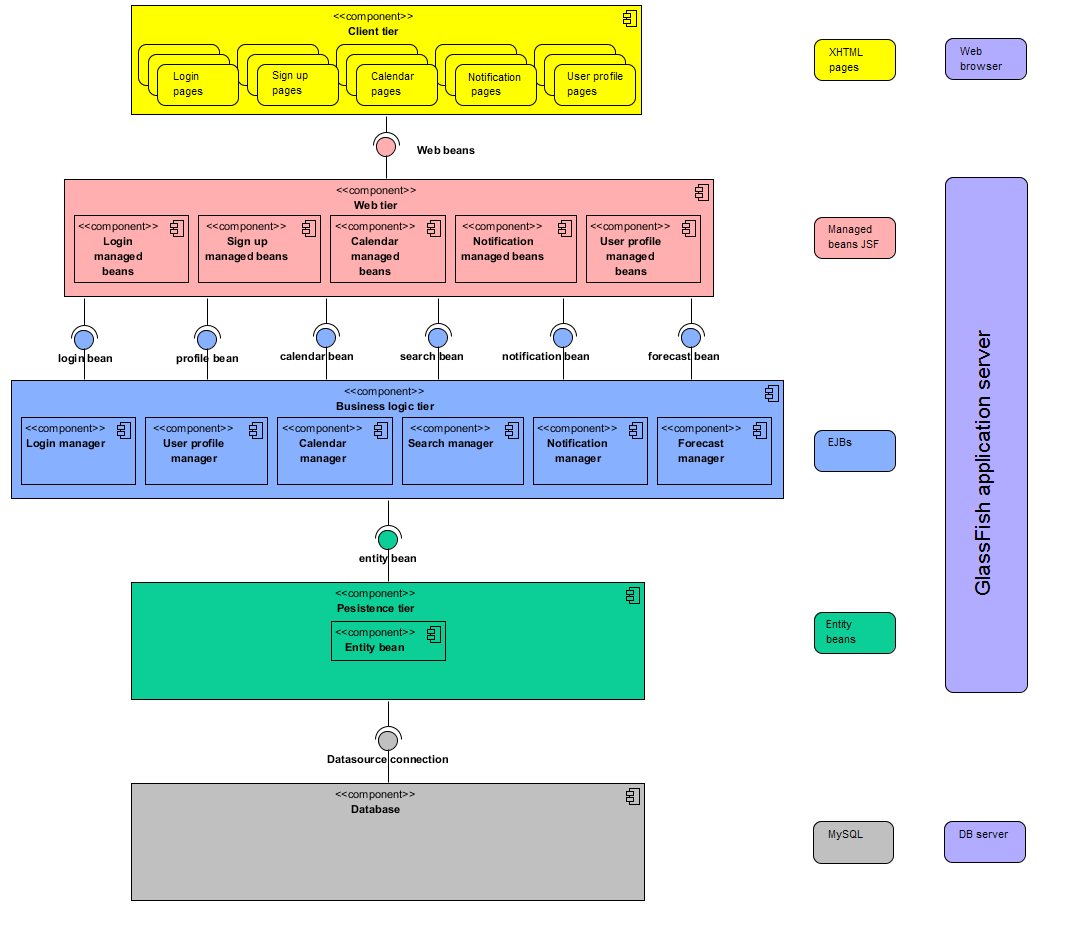
\includegraphics[width=\linewidth]{./images/general_architecture_design}
\caption[General architecture]{General architecture design}
\label{fig:general-architecture}
\end{figure}

The diagram represented in figure \ref{fig:general-architecture} represents our conceptual design of MeteoCal. This diagram depicts all the components of the designed software, by clarifying the logical separation between the tiers (Although we will build our application based on the 3-tier architecture).
It is clear that the user will interact with the XHTML pages, which in their side are implemented with beans to manage user interaction. This web interaction is then supported by the business tier, which holds on the information provided by the persistence layer. The persistence layer is the one in charge of the connection to the database and managing all the queries needed from the above layers.

\subsection{Client tier}
The client tier is composed of the XHTML pages that the system user will see. Actually this is strictly related to the Web Tier, so they will be described together in part \ref{part:detailed-software-design}.

\subsection{Web tier}
Web Tier is composed of the web beans. This tier receives requests from the user, interacts with the beans in the Business Logic tier and display data according to the user requests. Since we will be using JSF these beans are called Managed Beans.

\subsection{Business logic tier}
The business logic tier is composed of all the logic underlying our application; it is responsible of communicating with Web Tier and Persistence Tier. Its components are the EJB Beans.

\subsection{Pesistence tier}
The persistence tier is composed of the entity beans which represent the entities depicted from our RASD document and then further endorsed in our conceptual design. These entities are fundamental as they represent the connection to our database. Since in JEE we are interested in working in an object oriented environment, they represent a high level object view of the database of the application, which from its side connects to the Database Tier.

\subsection{Database}
The database is the tier that fiscally stores the information needed by our system. It's structure will be further explained in section \ref{sec:DatabaseModel}.

\section{System specifications}
The following table displays the technologies we will use during implementation. All of the technologies are free source technologies.

\noindent\begin{tabular}{| l | l |}
\hline	\emph{Component name}	&	\emph{Technology}	\\
\hline	Client tier \& Web tier	&	XHTML integrated with JSF	\\
\hline	Business tier			&	JEE with GlashFish AS	\\
\hline	Persistence tier \& Database tier	&	MySQL	\\
\hline
\end{tabular}

\clearpage
\part{Detailed software design}
\label{part:detailed-software-design}
In this part we provide a detailed description of the system architecture and intended implementation according the general structure already described in section \ref{sec:conceptual-design}.

\section{Database model}
\label{sec:DatabaseModel}
\subsection{Conceptual Design}
We developed the entity-relationship diagram following what we specified in the class diagram presented in the RASD. 
\paragraph{Notes}
\begin{itemize}
\item In the future the possibility of changing the user name could be implemented. Therefore we used an integer ID as the User primary key instead of the user name.In this way it will be simpler to manage future changes in the way the system manages user data. 
Emails can already be changed and thus weren't a suitable choice for the primary key.
\item Places have an ID as primary key. It's the id that identifies the specified city in Open Weather Map (the external service used to get forecasts). In this way it will be simpler to manage places and forecasts according to the external service.   
\end{itemize}

The User entity contains all the  user's personal information. A user has exactly one calendar. A user can create events and he may receive notifications.\
Calendar is a weak entity with respect to User because if a user is deleted from the database's records then there's no need  to keep track of its calendar. A calendar contains 0 or more events.\
An event is created by exactly one user and it's contained in at least one calendar (the one belonging to its creator). Events can generate notifications. An event is held in one Place (that may be unspecified) and has a related forecast, if available.\
A Place is the location of at least one Event. It can also be the object of some weather forecasts.\
Forecast is a weak entity with respect to Place because forecasts referring to places that are not in the DataBase make no sense. A forecast has to be used by at least one event, otherwise it would be useless.\
A notification has to have at least one receiver and it concerns exactly one event. ECN, BWA, SDP and Invite are heir classes of Notification because they share the basic structure but have to be managed in different ways.
\begin{figure}[p]
\centering
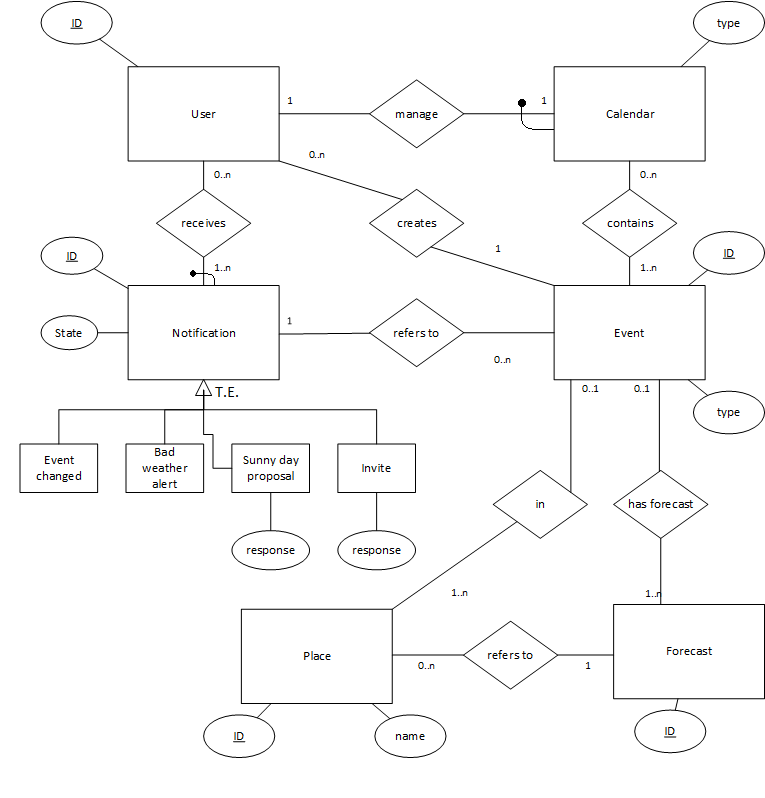
\includegraphics[width=\linewidth]{./images/ER}
\caption[ER]{Entity-Relationship diagram}
\label{fig:ER}
\end{figure}


\subsection{Logical design}
The logical design of the database represent its final representation. The diagram shows the different tables required to store MeteoCal data. Every attribute is a column of the table in which is declared. Every table may involve foreign keys. These are attributes that refer to another entity in the database, which is specified through its primary key. 
The LD diagram is derived from the ER diagram. Thus it presents the same structure for information. The relations specified in the ER are commonly specified in the LD diagram using foreign keys.\
We decided to remove the entity calendar. Conceptually it was useful but in practice, given that the relation with the user is 1:1 it can be omitted without any loss. A calendar table wouldn’t be reasonable because it would not contain enough information. We included the privacy setting of the calendar in the User table and connected directly users and the events their events.\
The User table contains all the personal details of a user. Its primary key is an integer generated automatically by the DBMS. 
Users are connected to their events with the Participates table. This table has a primary key composed by the couple user - event. The first one is a foreign key referring to the ID of the participant, the second is a foreign key with respect to the ID of the event.
The Event table contains alle the tuples representing events. Each tuple has a unique ID generated by the database. The attributes Place and Weather are optional because if the event is indoor users are not required to specify them. Place is a foreign key referring to the place ID. It specifies that each an event is held in 0 or 1 place. Weather is a foreign key referring to the forecast ID. It specifies the forecast which is shown to the user for the event.
The Forecast table has an integer primary key generated by the dbms. It has a foreign key that links the forecast to a specific place ID. 
The Place table has an integer primary key which is the city code used in the Open Weather Map. Therefore it has to be set by MeteoCal system and not automatically by the database.\
The Notification table contains all the different type of notification. The type is specified in the NotificationType attribute. We decided to store all the types in a single table because it simplifies the process of searching pending notifications for a given user. A notification has a primary key composed by the notification ID and a user ID. The notification ID is an integer generated by the database. The notification ID alone is not enough to identify a single notification because the same notification can be sent to multiple user and each of them may reply in a different way to it.\
\begin{figure}[p]
\centering
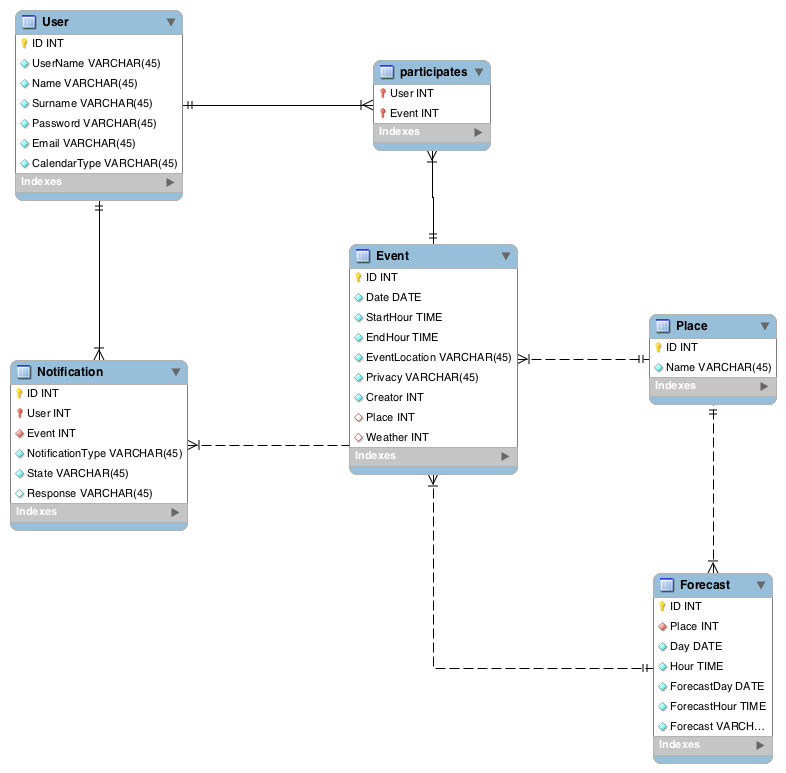
\includegraphics[width=\linewidth]{./images/Logic_view}
\caption[Logic view]{Logic view diagram}
\label{fig:Logic_view}
\end{figure}

\section{UX diagrams}
\label{sec:UXdiagrams}
\subsection{Unlogged user UX}
The following UX diagram describes the user experience related to the “first” part of the interaction with the user. Its focus is on how the user may accomplish the following actions: login, registration, logout. These actions refer respectively to functional requirements FR2, FR1 and FR3 (section “Managing User”).
The first page shown to the user is the Login Page, represented by the Login Screen. We marked it with the dollar symbol because this page is reachable from all the others. On the one hand, if the user hasn’t already performed the login, he is able to get back to the Login page from all the other pages accessible at that time (About page and Registration page). On the other if a logged user performs the logout he’s taken back to the login page. 
The Login screen has an input form where the user can insert username and password. If they are correct the user is taken to his Homepage (discussed in the second UX diagram), otherwise an error message will appear on the same page. From the Login page the user can reach the About page and the Register page.
The About page has the only function of explaining the purpose of MeteoCal system. Therefore it just shows some static text and allows the user to reach the Register page or to go back to the login.
The Register page contains an input form that allows the user to register into the MeteoCal system. When a user send a registration request his data are checked. If the system doesn’t detect any problem the registration is completed successfully. Personal data are stored and the user is taken to his homepage. If some data are missing or wrong the user remains on the Register page where an error message is shown.


\section{BCE diagrams}
Our system is composed by 3 main components, which will be implemented during implementation phase.
\begin{itemize}
\item Web component
\item Business logic component
\item Persistence component
\end{itemize}
In this section we describe all the subcomponents in a ``vertical way'', i.e. starting from a web component we will show how it interacts with the business logic component to achieve what it needs, and how the business logic interacts with the persistence component.

Figure \ref{fig:global_bce} represents the complete BCE diagram of our application. Each area of the application will be further explained in the following subsections.
\begin{figure}[p]
\centering
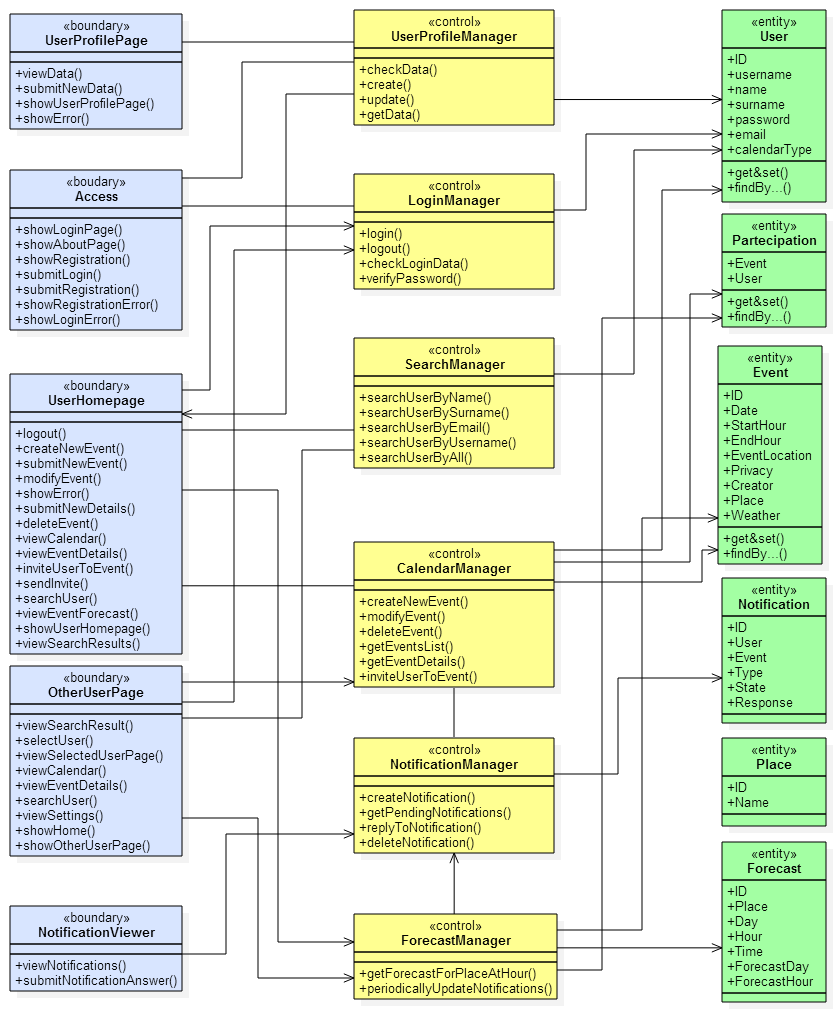
\includegraphics[width=\linewidth]{./bce/global_bce}
\caption[global bce]{Global BCE diagram}
\label{fig:global_bce}
\end{figure}
\clearpage

\subsection{User profiles managing}
The BCE diagram in figure \ref{fig:userProfile_bce} describes the main features of the user profiles managing (registration, login and data modifications). It displays all the parts of the MeteoCal system involved in carrying out this tasks.

The registration involves a controller that takes care of checking and storing user data in the User Entity. If the user sign-ups correctly he's taken to his homepage.  In this case the system doesn't perform  (quite clearly) any notifications control.

The login involves a Login Boundary to manage the interaction with the user, a controller that has to check the validity of the input data and the User Entity which clearly provide the necessary information. 
After the login has been successfully accomplished the controller calls the Home boundary (taking the user to its homepage) and activates the NotificationManager that will check for pending notifications.

From his homepage an user can reach his User Profile page, where he can update his data. That page uses the UserProfileManager to get the user data, shows them to user and waits for eventual modifications. When the user chooses to save the new data the boundary forwards them to the controller, that updates the underlying entity. 

\begin{figure}[h]
\centering
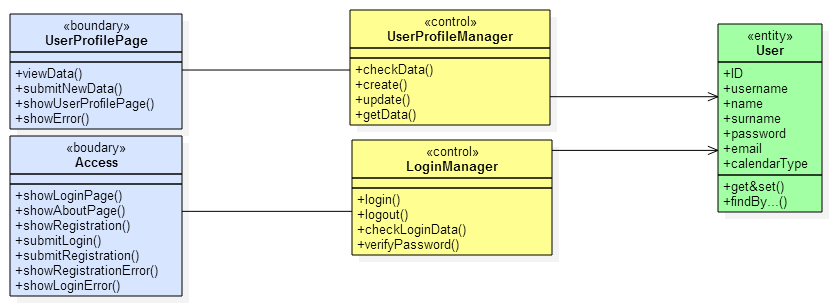
\includegraphics[width=\linewidth]{./bce/userProfile_bce}
\caption[user profile bce]{Signup, login and data update BCE diagram}
\label{fig:userProfile_bce}
\end{figure}

\subsection{Notification and forecasts managing}
The BCE diagram in figure \ref{fig:notification_bce} describes how the system manages the notifications and the weather forecasts.

The Notification viewer is a component that is used to show the pending notifications. The Notification viewer basically calls the Notification manager to obtain the list of pending notifications. Then it shows them to the user and eventually asks for a response that is given back to the manager. The notification manager can use the calendar manager to take care of the user response (for example if the user accepts an event invitation it will save the event in the user's calendar). Once viewed a notification can be deleted from the system.

A notification can be created by the calendar manager (for example if I create an event with some invitations the calendar manager will take care of creating the needed notifications) or by the forecast manager. The forecast manager has a periodical task that takes care of keeping updated forecasts for all the events, when it is necessary it creates the needed notifications (for example if one day before the event the system detects bad weather it will create a bad weather notify).
\begin{figure}[h]
\centering
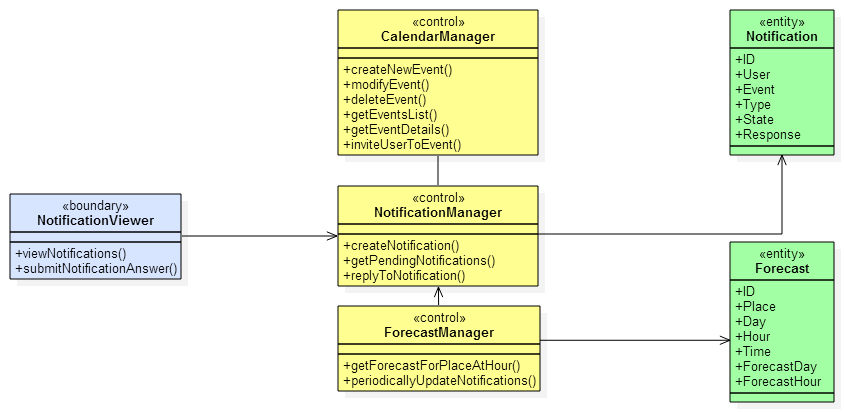
\includegraphics[width=\linewidth]{./bce/notification_bce}
\caption[notification bce]{Notifications and forecasts BCE diagram}
\label{fig:notification_bce}
\end{figure}

\subsection{Calendar browsing}
Figure \ref{fig:calendar_bce} contains the simplified BCE of calendar browsing (entities are not represented as they are visible in the global bce and further explained in section \ref{sec:DatabaseModel}).

The system has two similar boundaries for calendar browsing: one that shows the calendar of the actual user and one that is used to see the calendar of other users. They have some visual differences but they access the same controller as their task is quite similar.

The login manager is simply used to allow the user to log out of the system.
When browsing a calendar the boundaries access the calendar manager to obtain the needed informations on the events, and eventually to modify them.
When visualizing the details of an event the boundaries access the forecast manager to obtain the weather forecast for the event.
The search manager is used for searching another user (this can be done in order to view the user's calendar or to invite the user to an event).
\begin{figure}[h]
\centering
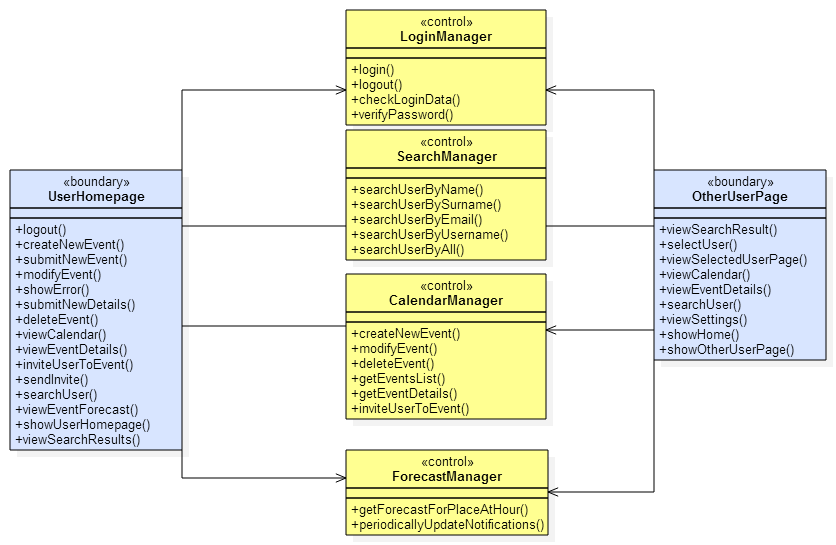
\includegraphics[width=\linewidth]{./bce/calendar_bce}
\caption[calendar bce]{Calendar BCE diagram}
\label{fig:calendar_bce}
\end{figure}

\section{Sequence diagrams}
TODO
In this section we provide some sequence diagrams that help understand how the system components work together in order to fulfill the functional requirements. We won't make a diagram for each functionality but will group them together in a sort of scenarios.

\subsection{Forecasts update and consequent notifications}
Figure \ref{fig:sequence_forecasts} contains the sequence diagram of a forecast update. The forecast manager has a periodical task that checks for weather updates, it searches for all the outdoor events that still have to take place, then it searches the places where these events take place and retrieve a forecast for each of them. Once updated the forecasts the manager look for the forecasts that went bad and eventually creates the needed notifications (the ones that have to be sent one day in advance and the ones that have to be sent three days in advance).
\begin{figure}[h]
\centering
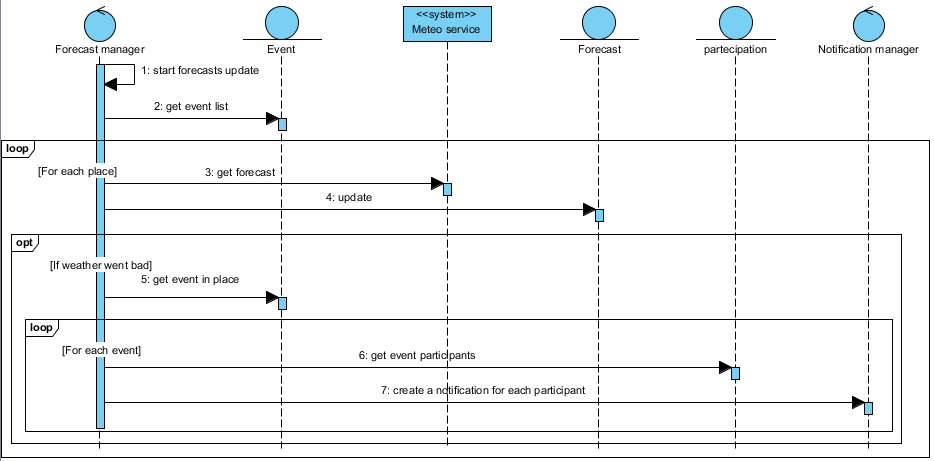
\includegraphics[width=\linewidth]{./images/sequence_forecast_update}
\caption[forecast update]{Forecasts update and conseqeunt notifications sequence diagram}
\label{fig:sequence_forecasts}
\end{figure}

\subsection{Signup and event creation}
\subsection{Login and event modification with an invite}

\section{Runtime view}
The diagram in figure \ref{fig:runtime_view} is the runtime view of MeteoCal project. The software will be released as a .ear so that it will be deployed on a JEE AS.
\begin{figure}[h]
\centering
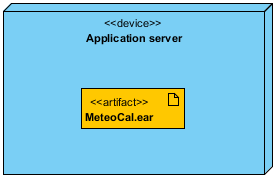
\includegraphics[width=0.5\linewidth]{./images/runtime_view}
\caption[runtime view]{Runtime view diagram}
\label{fig:runtime_view}
\end{figure}

\section{Deployment view}
The diagram in figure \ref{fig:deployment_view} represents how the components of the system will be deployed.
\begin{figure}[h]
\centering
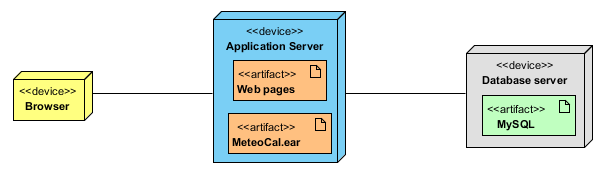
\includegraphics[width=\linewidth]{./images/deployment_view}
\caption[deploy]{Deployment view}
\label{fig:deployment_view}
\end{figure}

\clearpage
\part{Appendixes}
\label{part:appendixes}
\section{RASD modifications}
\subsection{Alloy model}
In the alloy model we stated that in our database we only keep track of one forecast per place (the most recent one). This fact is not true according to the database design and has to be removed. In fact we can have different events in the same place but on different days, so we need to have different forecasts.

\clearpage
\tableofcontents
\end{document}